\documentclass[a4paper,11pt]{article}

% Packages
\usepackage{listings}
\lstset{
    breaklines=true, % Break long lines
    language=SQL, % Set language for syntax highlighting
    basicstyle=\small, % Set the font size
    numbers=none, % No line numbers
    frame=single % Add a frame around the code
}
\usepackage{placeins}
\usepackage{float}
\usepackage{caption}
\usepackage[utf8]{inputenc}
\usepackage{amsmath}
\usepackage{graphicx}
\usepackage{geometry}
\usepackage{enumitem}
\geometry{a4paper, margin=1in}

% Title and Author
\title{Project 3}
\author{Ahmed Tlili, Leon Petrinos, Mathilde Peruzzo}
\date{\today}

\begin{document}

\maketitle

\section*{Relational Schema}
\begin{itemize}
    \item \textbf{Store}(\underline{s\_id}, s\_address, phone\_number, manager\_id UNIQUE NOT NULL)\\
        FOREIGN KEY(manager\_id) REFERENCES Employee(employee\_id)
    \item \textbf{Employee}(\underline{e\_id}, e\_name, s\_id)\\
        FOREIGN KEY(s\_id) REFERENCES Store(s\_id)
    \item \textbf{Manufacturer}(\underline{m\_id}, m\_name)
    \item \textbf{Product}(\underline{p\_id}, p\_name NOT NULL, unit\_price NOT NULL, description,\\ discount\_percentage, m\_id NOT NULL)\\
        FOREIGN KEY(m\_id) REFERENCES Manufacturer(m\_id)
    \item \textbf{Paint}(\underline{p\_id}, base, color)\\
        FOREIGN KEY(p\_id) REFERENCES Product(p\_id)
    \item \textbf{Tool}(\underline{p\_id}, type)
    \item \textbf{Has\_in\_stock}(\underline{p\_id}, \underline{s\_id}, quantity NOT NULL )\\
        FOREIGN KEY(p\_id) REFERENCES Product(p\_id)\\
        FOREIGN KEY(s\_id) REFERENCES Store(s\_id)
    \item \textbf{Customer}(\underline{email}, c\_name, c\_address NOT NULL)\\
        PRIMARY KEY(email)
    \item \textbf{Purchase}(\underline{p\_id}, amount NOT NULL, p\_date NOT NULL, p\_time NOT NULL)
    \item \textbf{Contains\_purchase}(\underline{p\_id}, \underline{product\_id}, quantity NOT NULL)\\
        FOREIGN KEY(p\_id) REFERENCES Purchase(p\_id)\\
        FOREIGN KEY(product\_id) REFERENCES Product(p\_id)
    \item \textbf{Instore}(\underline{p\_id}, \underline{e\_id})\\
        FOREIGN KEY(p\_id) REFERENCES Purchase(p\_id)\\
        FOREIGN KEY(e\_id) REFERENCES Employee(e\_id)
    \item \textbf{Online}(\underline{p\_id}, rating, delivery\_fee NOT NULL, email NOT NULL)\\
        FOREIGN KEY(p\_id) REFERENCES Purchase(p\_id)\\
        FOREIGN KEY(email) REFERENCES Customer(email)
\end{itemize}

\section*{Stored Procedure}

\begin{enumerate}[label=(\alph*)]
    \item This stored procedure increases the discount of products that havn't been sold in the past year by 10\%. The maximum discount is however a parameter to the procedure. 
    For example, if the maximum discount is 25\%, a product that already more than a 15\% discount (and less than 25\%) will have its discount updated to 25\%, not more. 
    Otherwise a product that has less than 15\% discount will get a 10\% discount increase.
    \item 
    \begin{lstlisting}
    CREATE OR REPLACE PROCEDURE DiscountInactiveProducts(IN max_discount INT)
    BEGIN
        DECLARE done INT DEFAULT 0;
        DECLARE current_pid INT;
        DECLARE current_discount INT;
    
        DECLARE product_cursor CURSOR FOR
            SELECT p_id, COALESCE(discount_pourcentage, 0)
            FROM Product
            WHERE COALESCE(discount_pourcentage, 0) < max_discount;
    
        DECLARE CONTINUE HANDLER FOR NOT FOUND SET done = 1;
    
        OPEN product_cursor;
    
        FETCH product_cursor INTO current_pid, current_discount;
    
        WHILE done = 0 DO
    
            IF NOT EXISTS (
                SELECT 1
                FROM Contains_purchase cp
                JOIN Purchase pur 
                ON cp.purchase_id = pur.p_id
                WHERE cp.product_id = current_pid
                    AND pur.p_date >= CURRENT DATE - 6 MONTHS
            ) THEN
                IF (current_discount + 10 > max_discount) THEN
                    SET current_discount = max_discount;
                ELSE 
                    SET current_discount = current_discount + 10;
                END IF;
    
                UPDATE Product
                SET discount_pourcentage = current_discount
                WHERE p_id = current_pid;
            END IF;
    
            FETCH product_cursor INTO current_pid, current_discount;
    
        END WHILE;
    
        CLOSE product_cursor;
    END
    \end{lstlisting}
    
    \item Calling the procedure: 
    Products with ids less than 25 before calling procedure: 
    Products with ids less than 25 after calling procedure:
\end{enumerate}

\section*{Application Program}

\section*{Indexing}

\subsection*{Index 1}

\begin{enumerate}[label=(\alph*)]
    \item 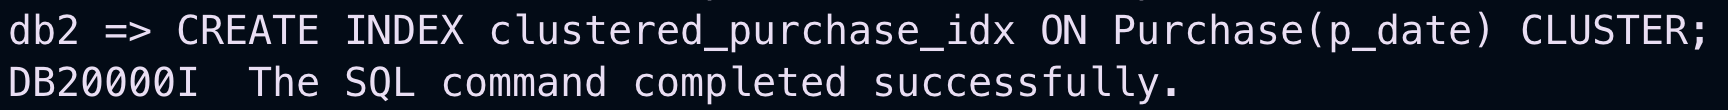
\includegraphics[width=0.9\textwidth]{images/idx1.png}
    \item A clustered index on purchase date in the Purchase table is beneficial because purchases are frequently analyed based on dates and date ranges. 
    Thus, sorting the purchases by date allows for efficient range queries, making it faster to access data for accounting purposes.
    An example query that would benefit from this index is the following:
    \begin{lstlisting}
        SELECT SUM(amount) AS total 
        FROM Purchase 
        WHERE p_date >= '01/01/2025' AND p_date <= '12/31/2025';
    \end{lstlisting}
    This above query computes the total revenue for the year 2025. With this clustered index, the database can quickly locate the first matching row, and perform a sequential scan to retrieve all rows within the specified date range, without needing to follow the pointers of other data entries (value + rid), as in a non-clustered index, which could often leed to more IO.
\end{enumerate} 

\subsection*{Index 2}
\begin{enumerate}[label=(\alph*)]
    \item 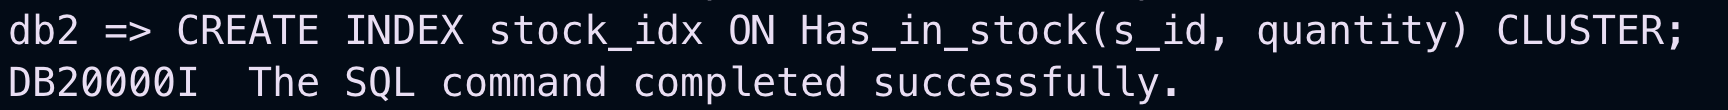
\includegraphics[width=0.9\textwidth]{images/idx2.png}
    \item This index is on the s\_id and quantity attribute of the Has\_in\_stock table. 
    It is useful for this application to efficiently identify products that are running low in stock in a specific store, which is crucial for inventory management.
    An example query that would benefit from this index is the following: 
    \begin{lstlisting}
        SELECT p_id 
        FROM Has_in_stock 
        WHERE s_id = 0 AND quantity < 5;
    \end{lstlisting}
    This query identifies all products of a particular store where the quantity of the product is very limited.
    The fact that it is a clustered index, again, allows for efficient range queries, making it faster to access data for inventory management purposes.
    It also makes sense to use a clustered index because the other attributes of the table are id's, which are certainly not needed in a sorted order. 
\end{enumerate}
\section*{Visualisation}

\subsection*{Vis 1}

\subsection*{Vis 2}

\section*{Creativity}


\end{document}

